\documentclass{article}

% Add search paths for input files
\makeatletter
\def\input@path{{../../../artisynth_core/doc/}{../../../artisynth_core/}{../../../artisynth_core/doc/texinputs/}}
\makeatother

\usepackage{amsmath}
\usepackage{framed}

%\usepackage{layout}
%\usepackage{showframe}
\input{artisynthDoc}
%\input{mathdefs}

\newcommand{\AS}{<ArtisynthRoot>}
\newcommand{\AM}{<ArtisynthModels>}
\newcommand{\BS}{<BatchsimRoot>}
\newcommand{\BM}{{\tt BatchManager}}
\newcommand{\BW}{{\tt BatchWorker}}
\newcommand{\BWs}{{\tt BatchWorkers}}

\begin{document}

\setcounter{tocdepth}{5}
\setcounter{secnumdepth}{3}

\title{The Batch Simulation Framework}
\author{Francois Roewer-Despres}
\setpubdate{Last update: June 26, 2018}

\iflatexml
\date{}
\fi

\maketitle

\iflatexml{\large\pubdate}\fi

\tableofcontents

% basic links to other docs: http://www.artisynth.org/doc/html/xxx/xxx.html#sec

\section{Introduction}

The Batch Simulation Framework (BatchSim) is a framework for running large batches of ArtiSynth simulations automatically and in parallel. The user specifies desired input configurations of a target model, then, for each configuration, BatchSim automatically runs a simulation and records desired outputs, with simulations optionally being performed in parallel.

The input configurations are specified using ArtiSynth's {\tt Property} mechanism, enabling BatchSim to be model-agnostic. Throughout this document, familiarity with {\tt Properties} is assumed. For an introduction to {\tt Properties}, see the \href{https://www.artisynth.org/Documentation/ModelingGuide}{ArtiSynth Modeling Guide}. For details, see the \href{https://www.artisynth.org/Documentation/MaspackRefManual}{Maspack Reference Manual}.

Throughout this document, assume that {\tt \AS} and {\tt \AM} denote the paths to the root folder of the ArtiSynth installation and the ArtiSynth Models extension, respectively. Given this, the root folder of BatchSim is {\tt \AM/src/artisynth/tools/batchsim} (referred to as {\tt \BS} for short).

BatchSim uses ArtiSynth's Jython interface. Throughout this document, familiarity with this interface is assumed. For details, see \href{https://www.artisynth.org/Documentation/MatlabAndJython}{Interfacing ArtiSynth to MATLAB and Jython}.

\section{Manager-worker architecture}

BatchSim treats all simulations it is meant to run as independent. That is, the output of one simulation cannot influence the input to another. As such, performing multiple simulations becomes an \href{https://en.wikipedia.org/wiki/Embarrassingly_parallel}{embarrassingly-parallel problem}. BatchSim exploits this potential for parallelism by adhering to the manager-worker architecture (a special case of the \href{https://en.wikipedia.org/wiki/Client?server_model}{client-server architecture}). By following this design pattern, BatchSim achieves terrific load balancing and serves as a general-purpose framework for automatically running simulations in either distributed or parallel fashion.

Within the context of BatchSim, the manager-worker architecture works as follows. One \BM\ process creates a number of ``tasks'' (based on user specifications), where each task represents a simulation to perform. The \BM\ then places these simulation tasks in a ``bag of tasks.'' Next, a certain number of \BW\ processes are created. Each \BW\ requests a task from the \BM, completes the task (by performing the simulation the task describes), records user-specified simulation results as output, and repeats until the bag of tasks is empty. The \BWs\ complete their tasks independently and in parallel (on a multicore system) or in a distributed fashion (on a multicomputer system), enabling a large \textbf{batch} of \textbf{sim}ulations to be completed in less time.
 
BatchSim includes a number of convenience methods for recording certain kinds of simple simulation outputs, but custom outputs can be specified by supplying custom \BWs\ to BatchSim (see Section \ref{custom:subclass}).

\section{Requirements and configuration}

\subsection{General}
\label{req:general}

BatchSim can run from within Eclipse or from the command line. However, the latter is \textit{significantly} easier since BatchSim requires at least two processes to be running simultaneously (one \BM\ and at least one \BW). This is possible but quite cumbersome to do in Eclipse, whereas using two separate command line consoles (or using background processes) makes running BatchSim from the command line trivial.

Whether running in Eclipse or from the command line, the following steps are necessary.

\begin{enumerate}

\item Ensure ArtiSynth is properly installed, and that all environment variables needed to run ArtiSynth are set. Note that Eclipse environment variables do not automatically create equivalent command line environment variables, and vice versa. Refer to the \href{https://www.artisynth.org/Documentation/InstallGuide}{ArtiSynth Installation Guide} for details.

\item Ensure {\tt \AS/classes} and {\tt \AM/classes} are on the Java class path. If additional custom classes are used, these must appear on the class path as well.

\item (Optional) In addition to hardcoded values, BatchSim can use random simulation inputs from a variety of \href{https://en.wikipedia.org/wiki/Probability_distribution}{probability distributions}. In this case, an additional Java library, called JDistlib, is required to run BatchSim. The JDistlib jar can be downloaded \href{http://jdistlib.sourceforge.net/}{here}. Once downloaded, ensure the jar file is on the Java class path.

\begin{sideblock}
Note: ArtiSynth does not ship with JDistlib because its license is slightly stricter than ArtiSynth's, leading to open-source incompatibilities. By using JDistlib, you agree to its license. \textbf{This only applies to using BatchSim with random simulation inputs (see next Note).}
\end{sideblock}

\begin{sideblock}
Note: JDistlib is \textbf{only} required for running probabilistic simulations \textbf{directly} in BatchSim. If you do not agree to JDistlib's license, then probabilistic simulations can still be approximated by first sampling from the desired probability distribution outside of BatchSim (using software such as R or Python) and then hardcoding the resulting values in BatchSim.
\end{sideblock}

\end{enumerate}

\subsection{Syntax highlighting}

The input configurations file to BatchSim will contain code written in a very simple programming language called the Property Specification Language (PSL) (see Section \ref{psl}). Syntax highlighting for PSL has been developed for Eclipse and Vim. See {\tt \BS/syntaxColoring} for instructions on how to get this feature up and running.

\begin{sideblock}
Note: at present, using the syntax highlighting in Eclipse is quite cumbersome. Using Vim is recommended.
\end{sideblock}

\section{Running BatchSim}

Running BatchSim from the command line is recommended (see Section \ref{req:general}), but running from Eclipse is also possible.

\subsection{General requirements}

To run BatchSim (from Eclipse or the command line), a number of files will be needed. Below is a summary of these file requirements. Details are given in the appropriate sections.

\begin{enumerate}

\item A target model (see Section \ref{psl:target-model}) with appropriate {\tt Properties} (see Section \ref{psl:prop-path}).

\item A \BW\ to customize simulation stop conditions and output recording (see Section \ref{custom}).

\item A very short Jython script for driving the custom \BW\ (see Section \ref{custom:jython}).

\item A file containing the desired input configurations (see Section \ref{psl}).

\item (Optional) Since BatchSim potentially produces many output files, an output folder may be convenient for organizational purposes, especially in post-processing (see Section \ref{misc:post}).

\begin{sideblock}
Note: simple defaults for the \BW\ and the Jython script exist (see Section \ref{custom:STBW}).
\end{sideblock}

\end{enumerate}

\begin{sideblock}
Note: for repeatable results while running probabilistic simulations, set the random number generator seed of the \BM\ (see {\tt -s} option of the \BM\ in Section \ref{running:advanced:BM}) and use the {\tt -disableHybridSolves} option to ArtiSynth when running \BWs\ (see Section \ref{running:CLI:BW}).
\end{sideblock}

\subsection{Minimal working example}

A minimal working example (MWE) of the entire BatchSim pipeline can be found in {\tt \BS/example}. It can be used as a way to try things out, or to make sure BatchSim is working properly. The only part of BatchSim not tested by this MWE by default is the proper functioning of JDistlib, which requires additional steps (see Section \ref{req:general}). To test this, use the file {\tt \BS/example/props-jdistlib.psl} as the input configuration file (see {\tt -f} option of the \BM\ in Section \ref{running:advanced:BM}).

This MWE was constructed as follows.

\begin{enumerate}

\item Decide on (or code up) a target model. In this case, \javaclass[artisynth.demos.mech]{SpringMeshDemo} was used for simplicity.

\item Decide on a {\tt Property} of the target model to configure during the simulations. In this case, the mass of the {\tt Particle} named {\tt pnt7} was used.

\item Write an input configurations file. In this case, two files were written. One is the ``default'' file, and is called {\tt props.psl}. The other file is used to (optionally) run probabilistic simulations, and is called {\tt props-jdistlib.psl}. To understand the contents of these files, see Section \ref{psl}.

\item Write a custom \BW\ to add a simulation stop condition as well as output recording. In this case, the custom \BW\ is {\tt SpringMeshDemoBatchWorker}. To understand what it is doing, see Section \ref{custom}.

\item Write a very short Jython script to drive {\tt SpringMeshDemoBatchWorker}. In this case, the Jython script is {\tt exampleBatchDriver.py}. To understand what it is doing, see Section \ref{custom:jython}.

\end{enumerate}

Feel free to use this MWE to test out the commands/concepts in the remaining sections.

\subsection{Running BatchSim from the command line}
\label{running:CLI}

With a given target model, \BW, Jython driver script, and input file, running BatchSim from the command line is done as follows.

\subsubsection{Running the \BM}
\label{running:CLI:BM}

To run the \BM, in one console window, execute the command

\begin{lstlisting}[]
  > java artisynth.tools.batchsim.manager.BatchManager -f <path-to-input-file>
\end{lstlisting}

This starts the \BM\ as a standalone process, and is the quickest and most lightweight option.

\begin{sideblock}
Note: by default, the \BM\ looks for an input file called {\tt props.psl} in the current working directory. If such a file exists (and is the input file you want the \BM\ to use) then the {\tt -f} option to the \BM\ can be omitted, as follows
\begin{verbatim}
  > java artisynth.tools.batchsim.manager.BatchManager
\end{verbatim}
\textbf{Unless otherwise noted, this is assumed to be the case in all subsequent examples involving the \BM.}
\end{sideblock}

Alternatively, execute the command

\begin{lstlisting}[]
  > artisynth -script <BatchsimRoot>/managerInit.py
\end{lstlisting}

This starts the \BM\ within an instance of ArtiSynth. This option is more heavyweight, but allows the \BM\ to verify that the contents of the input file represent valid {\tt Properties} for the target model. Doing this once is plentiful; it is thereafter much easier to run the \BM\ as a standalone application. To perform this validation, the {\tt -c} option must be passed to the \BM, and the target model must be loaded into ArtiSynth

\begin{lstlisting}[]
  > artisynth -model <target-model-classname> \
  >     -script <BatchsimRoot>/managerInit.py [ -c ]
\end{lstlisting}

\begin{sideblock}
Note: a \BM's validation of {\tt Properties} is not perfect. For each input configuration, the \BM\ will determine whether the target model has the appropriate {\tt Properties} and whether every \textit{hardcoded} {\tt Property} value is valid, but no such guarantee can be provided for \textit{probabilistic} {\tt Property} values, since these are not known ahead of time. Instead, the \BM\ checks that an \textit{arbitrary value} sampled from the probability distribution of each {\tt Property} is valid. Due to the inherent randomness in sampling probability distributions, this validation works on a best-effort basis only.

A \BW\ will also validate the {\tt Properties} for the target model, but unlike the \BM, this validation is only done as quickly as the \BW\ receives simulation tasks from the \BM\ (\textit{just-in-time} validation). Just-in-time validation does have the benefit of verifying \textit{probabilistic} {\tt Property} values, though, since at this point a random draw from the appropriate probability distribution has already been performed for the particular simulation the \BW\ is about to run, so the \BW\ can validate that particular value before running that particular simulation.

For these reason, most users prefer running the \BM\ as a standalone process (relying on just-in-time validation), rather than within an instance of ArtiSynth.
\end{sideblock}

\subsubsection{Running \BWs}
\label{running:CLI:BW}

Unlike the \BM, which is typically run as a standalone application, each \BW\ \textit{must} run within its own instance of ArtiSynth (in order to actually run simulations). The first step in running \BWs\ is to decide how many to run. Call this number $n$. The appropriate number of \BWs\ is entirely situation-dependent. For example, each \BW\ writes its output to a separate file (see Section \ref{misc:post:merging}). For small simulation batches, using a single \BW\ may work best, since it avoids the hassle of having to merge these separate output files. For larger batches, the parallelism offered by multiple \BWs\ is critical to speeding up completion times (hours vs. days).

\begin{sideblock}
Note: in general, each \BW\ uses of {\tt OMP\_NUM\_THREADS} number of threads (see the \href{https://www.artisynth.org/Documentation/InstallGuide}{ArtiSynth Installation Guide}). As such, it is generally most efficient to use approximately as many threads as the number of cores on your system, as this maximizes parallelism while minimizing context switching and/or thrashing.
\end{sideblock}

Once $n$ is set, execute the following command $n$ times to start $n$ \BWs

\begin{lstlisting}[]
  > artisynth -model <target-model-classname> \
  >     -script <path-to-Jython-driver-script>
\end{lstlisting}

There are essentially two ways of achieving this $n$-fold repetition.

\begin{enumerate}

\item Open $n$ consoles, and execute the command once in each console. This gives access to each individual \BW, but is quite tedious when $n$ is large.

\item (Recommended) In a single console, execute the command $n$ times in a loop. In this case, it is vital to run each \BW\ as a background process. In addition, the \BW\ console outputs can each be redirected to a separate file so they aren't interleaved in the console window. On a Unix-like system using Bash, this can be achieved with the following command

\begin{lstlisting}[]
  > for ((i = 0; i < n; i++)) ; do
  >     CONSOLE_OUT="$i"_console.log
  >     artisynth -model <target-model-classname> \
  >         -script <path-to-Jython-driver-script> >> $CONSOLE_OUT 2>&1 &
  > done
\end{lstlisting}

\end{enumerate}

If no errors have been made, BatchSim should now be running simulations as per the specifications in the input file. In addition, the simulations will run in parallel if $n > 1$.

\begin{sideblock}
Note: \textbf{performance is greatly improved} by running BatchSim without the ArtiSynth GUI. Typically, BatchSim is started once with the ArtiSynth GUI and with $n = 1$ to visually verify that the simulations are running as expected (using the correct target model, with desired inputs, etc.). After just one simulation, BatchSim is killed (see Section \ref{misc:kill}) and then restarted with ArtiSynth running in ``no GUI mode'' and with $n > 1$ to increase performance.

To run ArtiSynth in ``no GUI mode,'' add the {\tt -noGui} option to ArtiSynth. For example, to run a \BW\ in ``no GUI mode,'' execute the command
\begin{verbatim}
  > artisynth -noGui -model <target-model-classname> \
  >     -script <path-to-Jython-driver-script>
\end{verbatim}

Using the {\tt -noGui} option is usually coupled to low interactivity of the \BM\ (see option {\tt -i} of the \BM\ in Section \ref{running:advanced:BM}).
\end{sideblock}

\subsection{Running BatchSim from Eclipse}
\label{running:eclipse}

Running BatchSim from within Eclipse is similar to running it from the command line. One notable difference is that the working directory in Eclipse is a project root directory ({\tt \AS} for \BWs\ and {\tt \AM} for the \BM), so the path to the various files will have to be specified relative to those directories.

\subsubsection{Running the \BM}

To run the \BM\ \textbf{for the first time}: in the Eclipse {\sf Package Explorer}, right-click on the \javaclass[artisynth.tools.batchsim.manager]{BatchManager}{\tt .java} file in {\tt \BS/manager/} and select {\sf Run As > Java Application} from the context menu. This will start the \BM, but will immediately crash since the input file could not be found.

After running the \BM\ for the first time, right-click on the \javaclass[artisynth.tools.batchsim.manager]{BatchManager}{\tt .java} file and select {\sf Run As > Run Configurations...}. In the {\sf Run Configurations} window, click on the {\sf Arguments} tab, and add appropriate command line arguments (see Section \ref{running:CLI:BM}) in the text box labeled {\sf Program Arguments}. Then, click {\sf Apply} and {\sf Run}. Subsequently, the \BM\ can be started like any other Java program in Eclipse. Repeat this step whenever new command line arguments are desired.

\subsubsection{Running \BWs}

To run a \BW\ \textbf{for the first time}: in the Eclipse {\sf Console View}, right-click on arrow next to the window icon with a plus-sign in the top-right corner (see Figure \ref{fig:new-console}). From the menu that opens, select {\sf New Console View}.

\begin{figure}[t]
\begin{center}
\iflatexml
 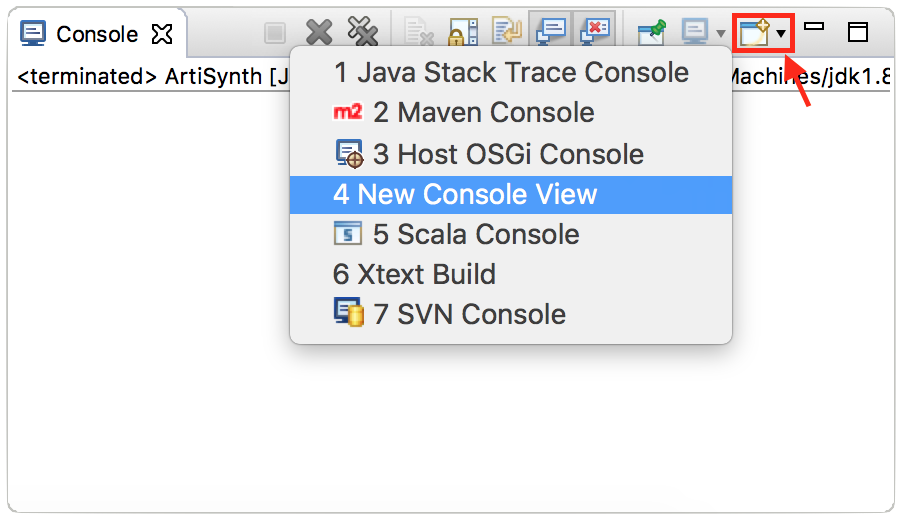
\includegraphics[]{images/batch-worker-launch-1}
\else
 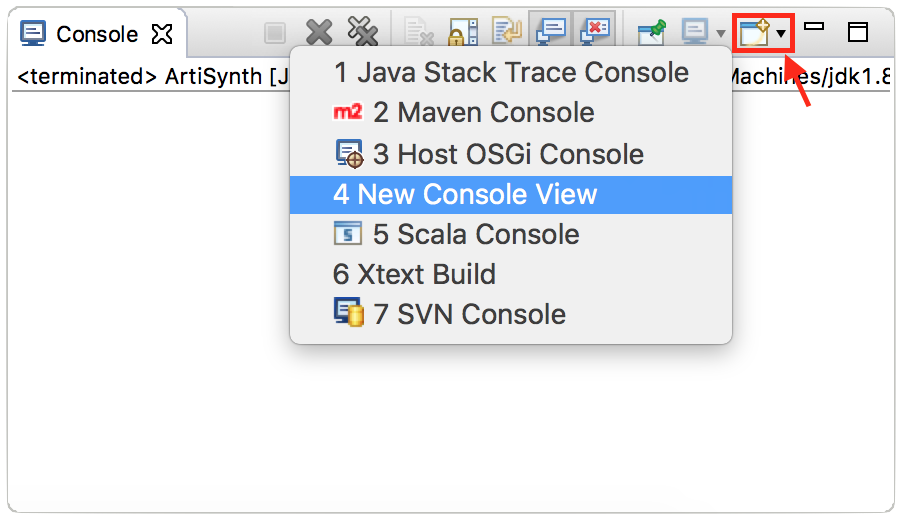
\includegraphics[width=6in]{images/batch-worker-launch-1}
\fi
\end{center}
\caption{Creating a new Console View in Eclipse.}
\label{fig:new-console}
\end{figure}

Next, return to the original console (where the \BM\ is running), and select the {\sf Pin Console} icon (a window with a green pin) in the top-right corner (see Figure \ref{fig:pin-console}). This will pin the \BM\ process to that console.

Finally, run the desired \BW\ by running ArtiSynth with the appropriate command line arguments for the \BW\ ({\sf Run As > Run Configurations... > Arguments > Program Arguments > Apply > Run}). Subsequently, the \BW\ can be started like any other Java program in Eclipse. Repeat this step whenever new command line arguments are desired.

\begin{figure}[t]
\begin{center}
\iflatexml
 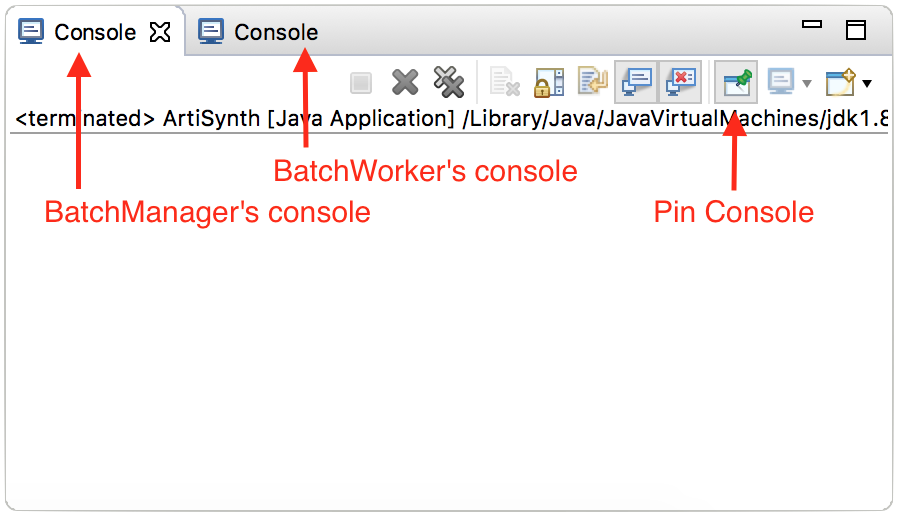
\includegraphics[]{images/batch-worker-launch-2}
\else
 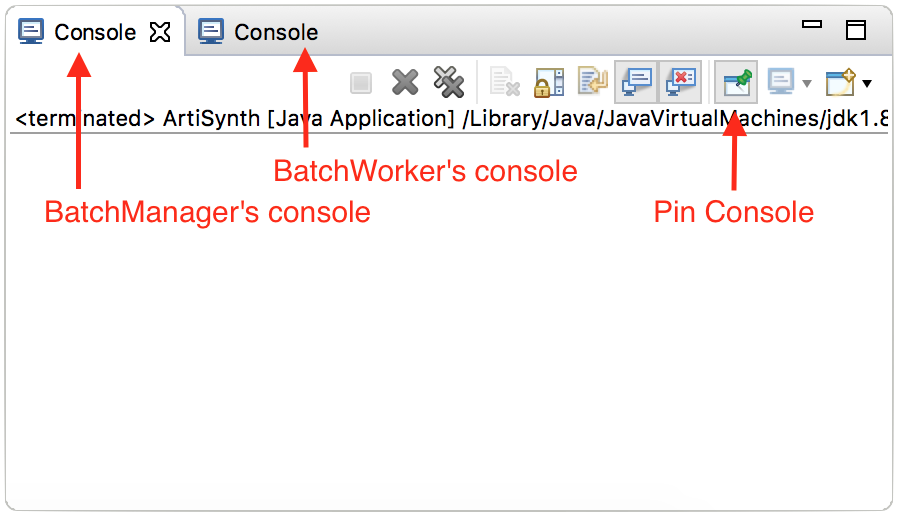
\includegraphics[width=6in]{images/batch-worker-launch-2}
\fi
\end{center}
\caption{Pinning a Console View in Eclipse.}
\label{fig:pin-console}
\end{figure}

\begin{sideblock}
Note: running more than one \BW\ from within Eclipse is not recommended, because Eclipse does not differentiate between instances of the same program when it comes to pinning program outputs in the Console Views. As such, the output from all but one \BW\ will not be visible in the Console Views (the program \textbf{will} run, but not in an accessible fashion). 
\end{sideblock}

\begin{sideblock}
Note: BatchSim can also run using Eclipse and the command line at the same time. For example, the \BM\ can run in Eclipse, while the $n$ \BWs\ can run from the command line.
\end{sideblock}

\subsection{Advanced BatchSim options}

The preceding examples (Sections \ref{running:CLI} and \ref{running:eclipse}) for running BatchSim present only the simplest and most common use cases. They allow BatchSim to run in its default mode. Additional modes and behaviours can be specified by appropriate command line arguments/options.

\begin{sideblock}
Note: running their respective program with the {\tt -help} option prints a summary of available options for both the \BM\ and \BWs.
\end{sideblock}

\begin{sideblock}
Note: for additional details, consult the Javadocs of \javaclass[artisynth.tools.batchsim]{BatchWorkerBase} and \javaclass[artisynth.tools.batchsim.manager]{BatchManager}.
\end{sideblock}

\subsubsection{Options to the \BM}
\label{running:advanced:BM}

At the time of writing, the options for the \BM\ are

\begin{description}

\item[{\tt -h,-help} ] \mbox{}

Prints a help message and exits.

\item[{\tt -f,-file <FILENAME>} ] \mbox{}

Reads the input configurations from file {\tt FILENAME}, which defaults to {\tt props.psl} in the current working directory. If {\tt FILENAME} is {\tt -}, reads from standard input (which forces an interaction level of 0; see {\tt -i} option).

\item[{\tt -m,-monteCarlo <N>} ] \mbox{}

If the input file (see {\tt -f} option) contains \textbf{only} probabilistic specifications, performs {\tt N} (which defaults to 1) \href{https://en.wikipedia.org/wiki/Monte_Carlo_method}{Monte Carlo} (i.e.\ random/probabilistic) simulations (see Sections \ref{psl:prob-spec} and \ref{psl:prop-spec:prob-spec}). \textbf{Otherwise, this option is ignored.}

\item[{\tt -p,-port <PORT>} ] \mbox{}

Binds the port to which the \BM\ socket is listening for requests from a \BW\ to {\tt PORT}, which defaults to 34365.

\item[{\tt -i,-interactionLevel <LEVEL>} ] \mbox{}

Sets the level of interaction with the user to {\tt LEVEL}, which defaults to 2 (unless {\tt -f -} is given; see {\tt -f} option). A \BM\ can run in ``interactive mode'' by initiating an interactive {\tt ArtisynthJythonConsole} session with the user. There are 3 levels of interaction. Level 0 means the \BM\ outputs nothing except error messages. Level 1 means the \BM\ outputs error and warning messages. Level 2 means fully interactive. In the latter mode, several builtin commands allow the user to interact with the \BM. These are

\begin{lstlisting}[]
  commands() -- output this list of commands
  progress() -- output progress information
  quit()     -- exit with status 0
  quit(st)   -- exit with status `st'
\end{lstlisting}

\begin{sideblock}
Note:  Low interactivity of the \BM\ is usually coupled to using the {\tt -noGui} option to ArtiSynth when running \BWs\ (see Section \ref{running:CLI:BW}).
\end{sideblock}

\item[{\tt -v,-debug} ] \mbox{}

Prints debugging (i.e.\ verbose) messages. This is independent of the interaction level (see {\tt -i} option).

\item[{\tt -r,-dryRun} ] \mbox{}

Reads the input file (see {\tt -f} option) and exits. This ensures the input file can be parsed without errors.

\item[{\tt -b,-bufferCap <CAP>} ] \mbox{}

Sets the maximum capacity of the buffer used to store created but unsent simulation tasks to {\tt CAP}. This is essentially the maximum size of the \BM's ``bag of tasks.'' {\tt CAP} defaults to $2^{20}$ (just over 1 million), but can be set to a larger value if more than that many simulations tasks will be created and the user is interested in knowing (before running all of them) the exact number of simulations to be run. On the other hand, it can be set to a smaller value if so many simulation tasks are being created that the JVM runs out of memory and crashes.

\item[{\tt -c,-checkProps} ] \mbox{}

If the \BM\ is running within an instance of ArtiSynth, verifies that the \textbf{currently-loaded} target model has all the {\tt Properties} listed in the input file (see {\tt -f} option), and that, for each such {\tt Property}, all the listed values are assignable to that {\tt Property} (see Section \ref{running:CLI:BM}).

\item[{\tt -d,-delimiter <CHAR>} ] \mbox{}

Sets the value delimiter character (see Section \ref{psl:prop-spec:comb-spec}) of the input file (see {\tt -f} option) to {\tt CHAR}, which defaults to {\tt \%}. Note that some characters are not recommended (high risk) and others are completely disallowed as the delimiter character (see {\tt -o} option; see Section \ref{psl:prop-spec:comb-spec}).

\item[{\tt -o,-riskyDelimOk} ] \mbox{}

Allows the use of delimiter characters (see {\tt -d} option) that are otherwise deemed too risky due to having syntactic significance (see Section \ref{psl:prop-spec:comb-spec}). Using risky delimiters may require escape characters (see Section \ref{psl:prop-spec:comb-spec}). At the time of writing, the illegal characters are: {\tt \{}, {\tt \}}, {\tt [}, {\tt ]}, {\tt \#}, {\tt (}, {\tt )}, and all digit and whitespace characters. At the time of writing, the risky characters are: {\tt =}, {\tt \textasciitilde}, {\tt "}, {\tt '}, {\tt @}, and {\tt \$}.

\item[{\tt -e,-epsilon <EPS>} ] \mbox{}

Sets the epsilon for comparing two doubles for equality to {\tt EPS}, which defaults to 0.0001.

\item[{\tt -s,-seed <SEED>} ] \mbox{}

Sets the seed for the random number generator to {\tt SEED}, or use no seed at all if {\tt SEED} is -1. {\tt SEED} defaults to -1.

\begin{sideblock}
Note: for truly repeatable results, setting this random seed is not enough. In addition, the {\tt -disableHybridSolves} option to ArtiSynth must be used when running \BWs\ (see Section \ref{running:CLI:BW}).
\end{sideblock}

\end{description}

\subsubsection{Options to \BWs}
\label{running:advanced:BW}

At the time of writing, the options for each \BW\ are

\begin{description}

\item[{\tt -h,-help} ] \mbox{}

Prints a help message.

\item[{\tt -n,-workerName <NAME>} ] \mbox{}

Sets the \BW's name to {\tt NAME}, which defaults to {\tt worker<PORT>}, where {\tt PORT} is supplied by the {\tt -p} option (or its default runtime value; see {\tt -p} option). Setting a unique name for each \BW\ is important, as it creates a one-to-one correspondence between each \BW\ and its output files, which prevents data corruption and facilitates post-processing (see {\tt -d}, {\tt -l}, and {\tt -f} options; see Section \ref{misc:post}).

\item[{\tt -d,-outputDirName <DIRNAME>} ] \mbox{}

Sets the \BW's output directory to {\tt DIRNAME}, which defaults to the current working directory. Having unique \BW\ names (see {\tt -n} option) allows each \BW\ to have its own (uniquely named) output file (see {\tt -l} and {\tt -f} options), and yet for all \BWs\ to share a single output directory. Having separate output files is critical to avoid data corruption, and sharing an output directory makes post-processing easier (see Section \ref{misc:post}).

\item[{\tt -e,-rerunSims <LIST>} ] \mbox{}

If a simulation fails, reruns that simulation using the time steps listed in {\tt LIST} until success is achieved. {\tt LIST} should be of the form {\tt <double>[[,...],<double>]} (a comma-separated list of doubles given as a single string). {\tt LIST} defaults to the empty list, meaning simulations are not rerun. Certain models, especially those containing finite-element models, are quite unstable and tend to cause simulation crashes. In this case, rerunning the simulation with one-tenth of the original time step can often increase stability enough to resolve the crash. However, running every simulation at that time step is not ideal, since smaller time steps require significantly more computation time. Hence the existence of this option. Since rerunning at one-tenth of the original time step is not always desired, providing a list of arbitrary doubles renders this options far more general.

\item[{\tt -l,-logFileName <FILENAME>} ] \mbox{}

Sets the \BW's log file name to {\tt FILENAME}, which defaults to {\tt <worker\_name>\_log.txt}, where {\tt worker\_name} is supplied by the {\tt -n} option. The log file is intended to store per-simulation logging information. Making use of this file is at the user's discretion (see {\tt addLogEntry()} in Section \ref{custom:subclass}).

\item[{\tt -f,-propValFileName <FILENAME>} ] \mbox{}

Sets the \BW's property-value file name to {\tt FILENAME}, which defaults to {\tt <worker\_name>\_propVal.txt}, where {\tt worker\_name} is supplied by the {\tt -n} option. The property-value file is intended to store the input configuration (i.e.\ the value of each {\tt Property} in the simulation task; see Section \ref{psl:sim-task}) used for each simulation run by that \BW. Making use of this file is at the user's discretion (see Section \ref{custom:subclass}).

\item[{\tt -p,workerReplyPort <PORT>} ] \mbox{}

Sets the \BW's \textbf{base} reply port to {\tt PORT}, which defaults to 23159. Note that the actual port used may be different if the port {\tt PORT} is already in use. In this case, the \BW\ will try binding each successive port (incrementing by one) until a port is successfully bound. This incrementing feature is extremely useful in practice, since starting $n$ \BWs\ will automatically cause $n$ successive ports to be bound, without having to explicitly pass a different port number to each \BW. In addition, since \BW\ names and log files (see {\tt -n}, {\tt -l}, and {\tt -f} options) are linked to the port number (by default), this feature ensures unique file names for each \BW\ by default (see {\tt -d} option).

\item[{\tt -m,managerHostName <HOSTNAME>} ] \mbox{}

Informs the \BW\ that the \BM's host machine's name is {\tt HOSTNAME}, which defaults to the \BW's localhost name or loopback address name (by default, BatchSim assumes the network connection between the \BM\ and the \BWs\ is local).

\item[{\tt -r,managerRequestPort <PORT>} ] \mbox{}

Informs the \BW\ that the \BM\ is listening for requests on port number {\tt PORT}, which defaults to 34365.

\end{description}

\begin{sideblock}
Note: custom \BWs\ can be given additional options (see {\tt otherParserOptions()} in Section \ref{custom:subclass}).
\end{sideblock}

\section{The Property Specification Language}
\label{psl}

Whereas \BWs\ are specifically designed to be customizable, the \BM\ is a complete program that is not intended to be modified by the user. Instead, the \BM's behaviour is influenced through the contents of the input file it receives from the user (see the {\tt -f} option of the \BM\ in Section \ref{running:advanced:BM}). This file contains the input configuration of every simulation that BatchSim should run for the current batch. These configurations are provided in a compact form in which the user specifies the values or probability distributions of various {\tt Properties} of a target model, which are known as property specifications. Properties specifications are written in a very simple programming language called the Property Specification Language (PSL). The input file simply contains a list of property specifications.

\subsection{The target model and {\tt Properties}}
\label{psl:target-model}

BatchSim is model-agnostic in the sense that it can run simulations for any {\tt RootModel} subclass, which BatchSim refers to as the \textbf{target model}. Like much of the ArtiSynth and Maspack codebases, this agnosticism is achieved by accessing model attributes through ArtiSynth's {\tt Property} mechanism, which is very general and widely used. Frequently, the input parameters that are to vary with each simulation are already {\tt Properties}, either of the target model itself, or else of one of its subcomponents (e.g.\ a finite-element model). Whenever an input parameter is not already a {\tt Property} of some component in the target model's component hierarchy, a {\tt Property} can readily be defined to ``wrap'' said input parameter so as to become a {\tt Property}. Refer to the \href{https://www.artisynth.org/Documentation/MaspackRefManual}{Maspack Reference Manual} for details on adding custom {\tt Properties} to any class, including a {\tt RootModel} subclass.

\subsection{Property paths}
\label{psl:prop-path}

Throughout this document, the terms ``property'', ``{\tt Property}'', and ``property path'' are used interchangeably and refer to both {\tt Properties} and property paths. Outside this document, a property path is simply a path from the target model to one of its subcomponents, followed by {\tt :} (a colon), followed by the name of a {\tt Property} of that component. For {\tt CompositeProperties}, sub-{\tt Properties} can be referenced by separating the name of the {\tt CompositeProperty} and its sub-{\tt Properties} with {\tt .} (a period). Refer to the \href{https://www.artisynth.org/Documentation/MaspackRefManual}{Maspack Reference Manual} for details on property paths.

\subsection{Simulation tasks and property-value pairs}
\label{psl:sim-task}

The \BM\ parses the input file and collects all property specifications listed therein. It then processes these property specifications in one of three ways (see Sections \ref{psl:comb-spec}, \ref{psl:prob-spec}, \ref{psl:hybrid}) to create simulation tasks. Each simulation task contains a list of {\tt Properties} and, for each, a particular value to which it should be set for that particular simulation. These are known as property-value pairs. Each value is a textual (i.e.\ string) representation of a value that can be assigned to the associated {\tt Property}. \textbf{The format of this string must be such that the {\tt PropertyInfo.scanValue(ReaderTokenizer)} method can scan it.}

There are two kinds of property specifications: combinatorial and probabilistic. As part of the property specification, the user either hardcodes the {\tt Property} values directly to create a combinatorial specification (see Section \ref{psl:prop-spec:comb-spec}), or else indicates the probability distribution from which to draw the values for the {\tt Property} to create a probabilistic specification (see Section \ref{psl:prop-spec:prob-spec}).

\subsection{Combinatorial property specifications}
\label{psl:comb-spec}

Here, a particular {\tt Property} is associated with a \textit{set} of values, and each value is assigned to the {\tt Property} in turn during successive simulations. Other {\tt Properties} are associated with different value sets in their own combinatorial specification. The \BM\ iterates through the values in all combinatorial specifications so as to perform an exhaustive/combinatorial search of the input space: each possible combination of property-value pairs for all combinatorial specifications is examined. Each simulation task consists of exactly one such combination. More formally, say there are $N$ such combinatorial specifications. Then, the general combinatorial algorithm is

\begin{lstlisting}[]
  for value1 in specification1.valueSet()
     for value2 in specification2.valueSet()
        // ...
           for valueN in specificationN.valueSet()
              createSimulationTask(value1, value2, ..., valueN)
           endFor
        // ...
     endFor
  endFor
\end{lstlisting}

\begin{sideblock}
Note: the actual algorithm is recursive (where {\tt // ...} represents the recursion), but it is easier to understand this ``unfolded'' version.
\end{sideblock}

\begin{sideblock}
Note: mathematically speaking, one simulation task is performed for each element in the $N$-ary \href{https://en.wikipedia.org/wiki/Cartesian_product}{Cartesian product} of all the value sets.
\end{sideblock}

\subsection{Probabilistic property specifications}
\label{psl:prob-spec}

Here, a particular \textbf{numeric} {\tt Property} is associated with a \textit{vector} of parametric probability distributions, with the size of the probability distribution vector equal to the size of the {\tt Property} vector. For a scalar numeric {\tt Property}, the probability distribution vector should contain a single entry. Other {\tt Properties} are associated with different probabilistic distribution vectors in their own probabilistic specification. If \textbf{only} probabilistic specifications are given, the manager creates simulation tasks by applying the \href{https://en.wikipedia.org/wiki/Monte_Carlo_method}{Monte Carlo} method. That is, for each probabilistic specification, all the distributions listed in its associated probability distribution vector are sampled, and a random-value vector is formed from the sampled values. These sampled vectors are then assembled into one simulation task (thus forming one Monte Carlo simulation task), and the process is repeated $M$ times, where $M$ is specified by the user (see the {\tt -m} option of the \BM\ in Section \ref{running:advanced:BM}). Formally, the algorithm is

\begin{lstlisting}[]
  for i in 1 to M
     vectors = new List()
     for specification in specificationsList
        sampledVector = new Vector()
        for distribution in specification.distributionVector()
           sampledVector.add(distribution.sample())
        endFor
        vectors.add(sampledVector)
     endFor
     createSimulationTask(vectors)
  endFor
\end{lstlisting}

\subsection{Running hybrid combinatorial/probabilistic simulations}
\label{psl:hybrid}

If \textit{at least one} probabilistic specification and \textit{at least one}  combinatorial specification are given, the combinatorial algorithm described above is used, but augmented with a check for the specification's type. If the specification is probabilistic, it is treated as if its distribution vector was a single combinatorial value (whose value just happens to be different with each combination). The end result is a hybrid algorithm between combinatorial and Monte Carlo

\begin{lstlisting}[]
  iterator = specificationsList.iterator()
  while iterator.hasNext()
     specification1 = iter.next()
     if specification1.type() is COMBINATORIAL
        for value in specification1.valueSet()
           specification2 = iterator.next()
           // ...
              createSimulationTask(value, ...)
           // ...
        endFor
     else // specification1.type() == PROBABILISTIC
        sampledVector = new Vector()
        for distribution in specification1.distributionVector()
           sampledVector.add(distribution.sample())
        endFor
        specification2 = iterator.next()
        // ...
           createSimulationTask(sampledVector, ...)
        // ...
     endIf 
  endWhile
\end{lstlisting}

\begin{sideblock}
Note: again, the actual algorithm is recursive (where {\tt // ...} represents the recursion), but it is \textit{much} easier to understand this ``unfolded'' version.
\end{sideblock}

\subsection{Property specifications}

\subsubsection{Property path syntax}

Whether combinatorial or probabilistic, each property specification begins with a double-quoted property path

\begin{lstlisting}[]
  "<property_path>"
\end{lstlisting}

where {\tt <property\_path>} must be a valid ArtiSynth property path (see Section \ref{psl:prop-path}), except for an optional component identifier set extension provided by BatchSim that allows multiple property paths to be grouped into a single specification (see Section \ref{psl:prop-spec:comp-id-set}).

\subsubsection{Combinatorial specification syntax}
\label{psl:prop-spec:comb-spec}

Each combinatorial specification must adhere to the following general format

\begin{lstlisting}[]
  "<property_path>" = <value_set>
\end{lstlisting}

where {\tt <value\_set>} must be of the form

\begin{lstlisting}[]
   { <delim><val1><delim> <delim><val2><delim> ... <delim><valN><delim> }
\end{lstlisting}

where {\tt <delim>} is a chosen value delimiter character ({\tt \%} by default; see the {\tt -d} option of the \BM\ in Section \ref{running:advanced:BM}). Each {\tt <valX>} consists of the entire string between two consecutive occurrences of {\tt <delim>} (including all whitespace (except the end-of-line character); see Section \ref{psl:prop-spec:general}), and is taken to be a string representation of a (valid) value for the associated {\tt Property}.

Some examples of valid combinatorial property specifications (when the delimiter character is the default {\tt \%}) are

\begin{lstlisting}[]
  "models/0/component/1:someProp.someSubProp" = {%1% %2% %3%}
  "color" = {%"red"% %"green"%}
  "someVectorProp" = {%[1 2 3]% %[4 5 6]%}
\end{lstlisting}

\begin{sideblock}
Note: the preceding example involving the {\tt color} property path illustrates why the default delimiter character is {\tt \%} instead of a more traditional character such as {\tt "} (double quote): if a {\tt Property}'s type is {\tt String}, the {\tt ReaderTokenizer} input to the {\tt PropertyInfo.scanValue(ReaderTokenizer)} method \textbf{must} be fed a double-quoted string, which means the values of this property specification would have had to be coded as {\tt ""red""} and {\tt ""green""} (if {\tt "} was the delimiter character). Clearly, this will not be parsed correctly. Similar arguments apply to using {\tt '} or {\tt ,} as the default delimiter character.

It \textbf{\textit{is}} possible to set the delimiter character to {\tt "}, but in this case the double quotes belonging in the value need to be escaped: {\tt "\textbackslash"red\textbackslash""} and {\tt "\textbackslash"green\textbackslash""}. This also requires passing the {\tt -o} option to the \BM\ (see Section \ref{running:advanced:BM}).
\end{sideblock}

\subsubsection{Probabilistic specification syntax}
\label{psl:prop-spec:prob-spec}

Each probabilistic specification must adhere to the following general format

\begin{lstlisting}[]
   "<property_path>" ~ <distribution_vector>
\end{lstlisting}

where {\tt <distribution\_vector>} must be of the form

\begin{lstlisting}[]
   [ <distribution1> <distribution2> ... <distributionN> ]
\end{lstlisting}

where the number of distributions listed between the pair of square brackets must match the size of the associated {\tt Property}'s data type. That is, for scalar-valued {\tt Properties}, a single distribution should be listed, whereas for vector-valued {\tt Properties}, the number of distributions listed should match the vector's size. Each {\tt <distributionX>} must be of the form

\begin{lstlisting}[]
  <Name_of_distribution>(<parameter1_value>, ..., <parameterN_value>)
\end{lstlisting}

where {\tt <Name\_of\_distribution>} is the \textit{non-quoted} string name of a probability distribution. To be valid, this name must match {\tt Distribution.toString()} for some \javaclass[artisynth.tools.batchsim.manager.DistributionSampler]{Distribution} value. Following the distribution name, a \textit{comma-separated} list of parameter values (integers or doubles, depending on the distribution) enclosed in one pair of parentheses should appear. The values must appear in the same order and be in the same quantity as specified by the corresponding \javaclass[artisynth.tools.batchsim.manager.DistributionSampler]{Distribution}, and each value must be a valid number for that parameter of that \javaclass[artisynth.tools.batchsim.manager.DistributionSampler]{Distribution} (note that integers can be coerced into doubles). 

Some examples of valid probabilistic property specifications are

\begin{lstlisting}[]
  "models/0/component/1:someScalarProp" ~ [ Normal(20.0, 1.5) ]
  "colorRGB" ~ [ Uniform(0, 1) Uniform(0, 1) Uniform(0, 1) ]
  "someVectorPropWithConstant2ndEntry" ~ [
     T(2)
     Uniform(1, 1)
     Normal(0, 1)
  ]
\end{lstlisting}

\begin{sideblock}
Aside: in probabilistic specifications, {\tt \textasciitilde} is borrowed from probability theory notation: if a random variable $X$ is distributed according to probability distribution $D$, then we write $X$ \textasciitilde\ $D$. Here, we augment this notation by using $\textbf{X}$ (the {\tt Property}) to represent a vector of random variables, and we specify one probability distribution, $D_i$, for each entry $i$ of $\textbf{X}$, notated as $\textbf{X}$ \textasciitilde\ [$D_1$ $D_2$ ... $D_n$].
\end{sideblock}

\subsubsection{General syntax}
\label{psl:prop-spec:general}

Some notes on the syntax (in terms of \href{https://en.wikipedia.org/wiki/Lexical_analysis#Tokenization}{tokens}) of property specifications follow. Unless otherwise indicated, syntax rules apply to both combinatorial and probabilistic property specifications.

\begin{enumerate}

\item The {\tt \#} token begins a comment. All characters between it and the next end-of-line character are ignored.

\item The {\tt <property\_path>} token must be double-quoted.

\item All tokens in any specification can be separated by an arbitrary number of whitespace characters. Thus, the following examples are all syntactically valid and semantically equivalent combinatorial property specifications

\begin{lstlisting}[]
  "models:prop" = { %val1% %val2% }
  "models:prop" = {%val1% %val2%}
  "models:prop"={%val1%%val2%}
  "models:prop" = {
     %val1%
     %val2%
  }
\end{lstlisting}

\item The value set of a combinatorial specification \textit{can} be empty: {\tt \{\}}. In this case, \textit{but only in this case}, the associated {\tt Property} will be assigned the value {\tt null} in \textit{all} simulation tasks.

\item Whitespace appearing in any double-quoted string will be considered part of the string token, \textbf{unless} it is an end-of-line character, which will cause the string to be split into multiple word tokens. This applies to both {\tt <property\_path>} and {\tt <valX>} tokens, and is caused by the \javaclass[maspack.util]{ReaderTokenizer} used to parse the input file. One exception to this rule is that non-end-of-line whitespace appearing \textit{within a component identifier set} of a {\tt <property\_path>} token is ignored (see Section \ref{psl:prop-spec:comp-id-set}).

\end{enumerate}

\subsubsection{Component identifier sets}
\label{psl:prop-spec:comp-id-set}

Within a {\tt <property\_path>}, a special set notation can be used as a shorthand to group multiple property paths into a single specification. This is useful when the multiple property paths would otherwise share the same value set (for combinatorial specifications) or distribution vector (for probabilistic specifications).

A target model has components, and all components have either a name or number (called a component identifier).

Within a {\tt <property\_path>}, instead of specifying a single component identifier at each level in the component hierarchy, a \textit{set} of identifiers can be specified (within a pair of curly braces). This set will be ``expanded'' in place by creating one (implicit) specification for each component identifier in the set. For example, the {\tt <property\_path>}

\begin{lstlisting}[]
  "models/{mySubComponent1 mySubComponent2}:prop"
\end{lstlisting}

will be expanded into

\begin{lstlisting}[]
  "models/mySubComponent1:prop"
  "models/mySubComponent2:prop"
\end{lstlisting}

This expansion works regardless of the property specification type: the value set (for combinatorial specifications) or distribution vector (for probabilistic specifications) is copied (re-instantiated) for each expanded {\tt <property\_path>}.

\begin{sideblock}
Note: the individual identifiers in a component identifier set must be separated by an arbitrary number of non-end-of-line whitespace characters.
\end{sideblock}

\begin{sideblock}
Note: since a component identifier set appears within a {\tt <property\_path>}, which is itself quoted by {\tt "}, the set cannot contain {\tt "} characters in it.
\end{sideblock}

\begin{sideblock}
Note: since components cannot be identified without an identifier, a component identifier set cannot be empty.
\end{sideblock}

When the component is identified by a number, that number is an integer. As such, an \textit{inclusive} range of such integers can be provided as yet an another shorthand. For example, the {\tt <property\_path>}

\begin{lstlisting}[]
  "models/{[0-2] [24-25]}:prop"
\end{lstlisting}

will be expanded into

\begin{lstlisting}[]
  "models/0:prop"
  "models/1:prop"
  "models/2:prop"
  "models/24:prop"
  "models/25:prop"
\end{lstlisting}

\begin{sideblock}
Note: an arbitrary number of whitespace characters can separate the individual characters within the range.
\end{sideblock}

\begin{sideblock}
Note: the first integer specified in a range must be less than or equal to the second integer in the range, but separate ranges need not be listed in increasing order.
\end{sideblock}

The expansion of a component identifier is done in place. That is, the substring delimited by the curly braces will be exactly replaced by each identifier listed in the set. For example, the {\tt <property\_path>}

\begin{lstlisting}[]
  "models/comp{   [0-2] [24-25] }onent:prop"
\end{lstlisting}

will be expanded into

\begin{lstlisting}[]
  "models/comp0onent:prop"
  "models/comp1onent:prop"
  "models/comp2onent:prop"
  "models/comp24onent:prop"
  "models/comp25onent:prop"
\end{lstlisting}

and the {\tt <property\_path>}

\begin{lstlisting}[]
  "models/{ left right top }_comp:prop"
\end{lstlisting}

will be expanded into

\begin{lstlisting}[]
  "models/left_comp:prop"
  "models/right_comp:prop"
  "models/top_comp:prop"
\end{lstlisting}

The identifiers in a component identifier set can in fact be component paths or path fragments as well. For example, the {\tt <property\_path>}

\begin{lstlisting}[]
  "models/{comp0/1 comp2/3}:prop"
\end{lstlisting}

will be expanded into

\begin{lstlisting}[]
  "models/comp0/1:prop"
  "models/comp2/3:prop"
\end{lstlisting}

Finally, multiple \textit{sequential} component identifier sets can be specified within a single {\tt <property\_path>}, and these will be expanded in a combinatorial fashion. For example, the {\tt <property\_path>}

\begin{lstlisting}[]
  "models/comp{0 1}/{2 3}:prop"
\end{lstlisting}

will be expanded into

\begin{lstlisting}[]
  "models/comp0/2:prop"
  "models/comp0/3:prop"
  "models/comp1/2:prop"
  "models/comp1/3:prop"
\end{lstlisting}

However, at the time of writing, BatchSim does \textbf{not} support nested component identifier sets. For example, the {\tt <property\_path>}

\begin{lstlisting}[]
  "models/comp{[0-1] {3 7 9}}:prop"
\end{lstlisting}

is \textbf{\textit{not}} valid and will not be expanded.

\subsubsection{Decorators}

Sometimes, it may be useful to specify a property specification as probabilistic, but then pre-sample from its distribution vector a certain number of times, say $k$, and treat these $k$ values as though they were values in a combinatorial value set. In other words, the property specification is specified as probabilistic, but we sample from it $k$ times, and then treat the resulting values as the $k$ values of the value set of a combinatorial property specification.

Similarly, we may want to specify as property specification as combinatorial, but instead of iterating deterministically through its value set to created simulation tasks, we may want to randomly sample from this set. Furthermore, we may want each value to have a different probability of being sampled. In other words, the property specification is specified as combinatorial, but we treat its value set as the support of a \href{https://en.wikipedia.org/wiki/Probability_distribution#Discrete_probability_distribution}{discrete probability distribution}, and then sample from this distribution as if the property specification was probabilistic.

BatchSim supports both of these features through \href{https://en.wikipedia.org/wiki/Decorator_pattern}{decorators}. As the name implies, these objects ``decorate'' a property specification to modify its interpretation. The syntax is as follows.

For combinatorially-decorated probabilistic specifications

\begin{lstlisting}[]
  @COMB(k) <probabilistic_property_specification>
\end{lstlisting}

leads to sampling the distribution vector of the specification $k$ times.

\begin{sideblock}
Note: to have repeatable results, consider fixing the seed of the \BM's random number generator (see {\tt -s} option to the \BM\ in Section \ref{running:advanced:BM}).
\end{sideblock}

For probabilistically-decorated combinatorial specifications

\begin{lstlisting}[]
  @PROB <combinatorial_property_specification>
\end{lstlisting}

leads to uniform sampling of the value set, while

\begin{lstlisting}[]
  @PROB(p1, p2, ..., pN) <combinatorial_property_specification>
\end{lstlisting}

leads to sampling with value-specific probabilities. Here, the usual constraints on discrete probability distributions, namely $\Sigma{p_i} = 1$ and $p_i \geq 0$, $i = 1,2,\dots,N$, must hold.

\begin{sideblock}
Note: the first form is just a shorthand for the second form, with $p_i = \frac{1}{N}$, $i = 1,2,\dots,N$.
\end{sideblock}

\begin{sideblock}
Note: the number of values in the value set \textbf{must} match the number of arguments to the {\tt @PROB} decorator.
\end{sideblock}

\begin{sideblock}
Note: at the time of writing, BatchSim does not support the addition of more than one {\tt @PROB} or {\tt @COMB} decorator to a single property specification.
\end{sideblock}

Sometimes it may be useful to have a property specification that exists solely for triggering control structures (see Section \ref{psl:control-struct}), rather than as a simulation input. But property specifications that don't correspond to a real {\tt Property} in the target model result in the \BWs\ throwing a runtime error. The only way around this would be to add a new ``phony'' {\tt Property} to the target model. This is obviously not very elegant and needlessly clutters the target model's code. Instead, a third kind of decorator exists, the {\tt @PHONY} decorator, which simply flags the property specification as phony. The \BM\ never passes any phony {\tt Properties} to the \BWs, which resolves the runtime error problem, but phony property specifications can still be used in the input file to trigger control structures.

\begin{sideblock}
Note: any property specification (whether otherwise decorated or not) can be \textbf{prepended} by \textit{at most one} {\tt @PHONY} decorator.
\end{sideblock}

\subsection{Control structures}
\label{psl:control-struct}

At the time of writing, property specifications can be affected by three control structures: {\tt skip} statements, {\tt redef} (i.e.\ redefinition) statements, and Jython code blocks. These structures are useful for removing certain combinations of input values that would otherwise be discarded as invalid simulations in post-processing. The power of using these structures comes from the fact that they save valuable computation time by not running simulations that will end up being discarded anyways. In addition, they simplify post-processing, because discarding specific pieces of data later on may be non-trivial, and may require manual intervention (although this depends on how the output data is recorded).

\begin{sideblock}
Note: because they can interact in complex and very subtle ways, very little checking is done to ensure valid use of these control structures prior to running simulations. For example, multiple {\tt redef} statements can ``cascade,'' where one is triggered, which redefines some other {\tt Property}, which later triggers yet another. Although this is valid, and even encouraged in many cases, no checks are made to ensure nothing is done incorrectly. Instead, task creation proceeds assuming everything will work out, and only if an error is detected during task creation will a meaningful error message be given.
\end{sideblock}

\subsubsection{{\tt skip} statements}
\label{psl:control-struct:skip}

A {\tt skip} statement is a list of \textit{combinatorial} property specifications, each of which has to have a property path that has already been defined at some earlier point in the input file (possibly with a different value set; the ``identity'' of property specifications is tied to the property path). A {\tt skip} statement causes simulations to be skipped. Specifically, it skips all simulations where each {\tt Property} listed in the {\tt skip} statement has a current value equal to any one of the values listed in its value set. That is, multiple property specifications listed together in the same {\tt skip} statement are logically ANDed, and, within each property specification, the values in its value set are logically ORed. This is called a {\tt skip} match. The syntax of a {\tt skip} statement is the keyword {\tt skip} followed by a list of \textbf{undecorated, combinatorial} property specifications (called the {\tt skip} block), followed by the keyword {\tt end}. For example

\begin{lstlisting}[]
  "prop1" = {%0% %1% %2%}
  "prop2" = {%3% %4% %5%}
  skip
     "prop1" = {%1% %2%}
     "prop2" = {%3% %4%}
  end
\end{lstlisting}

will skip all simulations where ({\tt prop1} = {\tt 1} OR {\tt prop1} = {\tt 2}) AND ({\tt prop2} = {\tt 3} OR {\tt prop2} = {\tt 4}), but allow all others (i.e.\ the pairs ({\tt 0}, {\tt 3}), ({\tt 0}, {\tt 4}), ({\tt 0}, {\tt 5}), ({\tt 1}, {\tt 5}), and ({\tt 2}, {\tt 5}) are all allowed).

\subsubsection{{\tt redef} statements}

{\tt redef} statements are composed of two blocks. The syntax is the keyword {\tt redef} followed by a list of property specifications, which may be combinatorial or probabilistic, and decorated or not (called the {\tt redef} block), followed by the keyword {\tt when}, followed by a list of \textbf{undecorated, combinatorial} property specifications (called the {\tt when} block), followed by the keyword {\tt end}.

The {\tt when} block is similar to the {\tt skip} block of the {\tt skip} statement, except that instead of skipping simulation tasks that match the block, it triggers the redefinition of the property specification(s) in the {\tt redef} block. ``Redefinition'' means that the property path stays the same, and so refers to the same {\tt Property} of the target model, but some other part of the property specification changes. The change can be anything: adding a decorator, changing the values in the value set, changing the probability distributions in a distribution vector, changing the size of the value set or distribution vector, changing the property specification from combinatorial to probabilistic, or anything else.

A list of these redefinable property specifications should appear in the {\tt redef} block. This list is just a shorthand: implicitly, there is one separate and completely independent redefinition for each property specification listed in the {\tt redef} block. As such, it would be equivalent to having one redefinition with the same {\tt when} block for each property specification listed in the {\tt redef} block. One catch: \textbf{every} property specification listed in the {\tt redef} block must be initially defined (in the input file) \textbf{after} every specification listed in the {\tt when} block.

\begin{sideblock}
Aside: we can think of the contents of the input file as a directed graph where each property specification is a node, and where there is a \textit{directed} edge from one property specification to another if the former appears immediately before the latter in this file. Then, a topological sort of the resulting directed acyclic graph (DAG) would place the property specifications in the same order as they appear in the input file. With this in mind, we can think of a {\tt redef} statement as introducing several more directed edges to the DAG. Each such edge starts at a property specification in the {\tt when} block and ends at a property specification in the associated {\tt redef} block. The {\tt redef} statement, then, is valid if and only if the graph that results from the introduction of these new edges is still a DAG (i.e.\ has no cycles). This is done to prevent cyclical redefinitions, which are usually hard to get right, and often cause infinite loops unless extreme care is taken to avoid them.
\end{sideblock}

{\tt redef} statements become extremely useful when combined with phony property specifications acting as flags. For example

\begin{lstlisting}[]
  @PHONY "prop1" = {%LOW% %HIGH%} # The flag is defined before the "real" properties.
  "prop{2 3}" = {} # prop2 & prop3 are initially set to null (to be redefined later).
  redef
     "prop2" = {%1% %2%}
     "prop3" = 
  when
     "prop1" = 
  end
  redef
     "prop2" = {%9% %10%}
     "prop3" = 
  when
     "prop1" = 
  end
\end{lstlisting}

Here, {\tt prop1} acts as a flag which makes some other properties, namely {\tt prop2} and {\tt prop3}, have values that are either low or high in tandem. This effectively skips simulations where one has a low value while the other has a high value, which (in this example) we would want to discard as invalid.

\begin{sideblock}
Note: since the effect of {\tt skip} and {\tt redef} statements is the same (discarding unwanted simulations), these two structures are effectively equivalent. Indeed, they simply represent different ways of expressing some discard behaviour/logic, and one can always be defined in terms of the other. However, since the logic may be much more complicated to express with one compared to the other, both are made available for convenience.
\end{sideblock}

\subsubsection{Jython code blocks}

Jython code blocks are different from {\tt skip} and {\tt redef} statements in that they are not standalone statements. Instead, they must occur within a {\tt skip} or {\tt when} block. They act as an additional way in which {\tt skip} or {\tt when} matches can be detected. This can be useful, for example, to match conditional on the value of a probabilistic property specification, which are not allowed in {\tt skip} and {\tt when} blocks. In fact, Jython code blocks can entirely replace the combinatorial matching described above. The advantage of the combinatorial matching, however, is in terms of (1) a convenient syntax, and (2) \textbf{noticeably faster computation time} on the part of the \BM\ (the \BWs\ are unaffected).

\begin{sideblock}
Note: the computational slowdown comes from the fact that, rather than executing everything in Java, the \BM\ has to load the Jython code into a Jython interpreter and then relinquish control to the interpreter, which runs the Jython code before eventually returning control to the \BM.

\textbf{Although the computational slowdown is noticeable, it is \textit{rarely} significant enough to cause problems.} This is because the \BM\ creates simulation tasks (to fill its bag of tasks) in a separate thread than the one listening for task requests from the \BWs. A slowdown will therefore only affect the overall speed of BatchSim if simulation runtimes are faster than task creation times. This is very unlikely, unless the target model is extremely simple and there are a lot of Jython code blocks in the input file.
\end{sideblock}

The syntax of a Jython code block is the keyword {\tt jython} followed by a list of arbitrary lines of Jython code, each of which must be prepended by a {\tt \$}, followed by the keyword {\tt end}. Within the Jython code, two special functions are exposed.

\begin{description}

\item[{\tt get()} ] \mbox{}

Takes a string representing a property path, and returns the current value of the property specification with that property path (as a string), or {\tt None} if the value is not set.

\item[{\tt return\_value()} ] \mbox{}

Takes a boolean and returns nothing. {\tt return\_value()} is a callback that passes the given value back to the \BM. If the Jython code block should trigger a match (either in a {\tt skip} or {\tt when} block), then {\tt return\_value(True)} should be called. Otherwise, {\tt return\_value(False)} should be called.

\begin{sideblock}
Note: calling {\tt return\_value()} multiple times within a single Jython code block is not permitted.
\end{sideblock}

\begin{sideblock}
Note: if a {\tt skip} or {\tt when} block contains both Jython code blocks and combinatorial property specifications, then all of them must match for an overall match to be established.
\end{sideblock}

\end{description}

As an example of using Jython code blocks, consider

\begin{lstlisting}[]
  "prop1" = {%0% %1% %2%}
  "prop2" = {%3% %4% %5%}
  skip
     jython
        $prop1_val = get("prop1")
        $return_value(prop1_val in ["1", "2"])
     end
     "prop2" = {%3% %4%}
  end
\end{lstlisting}

This is identical to the example {\tt skip} statement shown in Section \ref{psl:control-struct:skip}, \textbf{except that it will be computationally slower}.

\begin{sideblock}
Note: Although it may not be apparent in this simple example, the (often slight) computation slowdown of the Jython code blocks may well be worth it, since, in more complicated use cases, using only the basic functionality of {\tt skip} or {\tt redef} statements may be extremely cumbersome/bug-prone. In general, the basic {\tt skip} and {\tt redef} statements should be considered ``accelerated'' special cases provided by BatchSim.
\end{sideblock}

In addition to the above Jython code block syntax, Jython one-liners can be specified by appending an additional {\tt \$} to the end of the one line of Jython code (the {\tt end} keyword must still be present). For example, the following is identical to the previous example

\begin{lstlisting}[]
  "prop1" = {%0% %1% %2%}
  "prop2" = {%3% %4% %5%}
  skip
     jython $return_value(get("prop1") in ["1", "2"])$ end
     "prop2" = {%3% %4%}
  end
\end{lstlisting}

\section{Customizing \BWs}
\label{custom}

Whereas the \BM's behaviour is modified using the input file, the \BWs\ are designed to be customized by sublcassing \javaclass[artisynth.tools.batchsim]{BatchWorkerBase}.

\subsection{What \BWs\ do}

\javaclass[artisynth.tools.batchsim]{BatchWorkerBase} is an abstract class that does most of the heavy-lifting required of a \BW. Specifically, \javaclass[artisynth.tools.batchsim]{BatchWorkerBase} handles the communication between a \BW\ client and a \BM\ server. It also handles, upon receiving a simulation task from the \BM, setting the new value of the appropriate {\tt Properties} of the target model. Finally, it takes care of running all simulations, including potential reruns (see {\tt -e} option the \BW\ in Section \ref{running:advanced:BW}).
 
The abstract \javaclass[artisynth.tools.batchsim]{BatchWorkerBase} class uses the \href{https://en.wikipedia.org/wiki/Template_method_pattern}{template method pattern}, which means it leaves ``holes'' in its methods by calling abstract sub-methods. Concrete (i.e.\ non-abstract) subclasses should override these sub-methods to add custom behaviour to the \BW. The {\tt run()} method is where most of these abstract methods get called. Since the {\tt run()} method is quite complex, a pseudo-code of the implementation is provided here, so that the order in which these abstract methods get called, and what happens between those method calls, is made very clear.

\begin{lstlisting}[]
  run():
     startLogSession() // For a subclass to override.
     setUpStopConditionMonitor() // For a subclass to override.
     while requestSimTask() != NULL: // While there are simulation tasks left.
        success = false // Set to true once a simulation succeeds (no error occurred).
        myNumSimsAttempted = 0 // For a subclass to know how many reruns happened.
        timeStepsToTry = List(targetModel.getMaxStepSize()) // All the potential ...
        timeStepsToTry.addAll(myRerunList) // ... time steps to try before giving up.
        while !success && !timeStepsToTry.isEmpty():
           myLastStepSizeUsed = timeStepsToTry.removeFirst() // For a subclass to know
           myNumSimsAttempted++ // For a subclass to know.
           reset() // Reset the target model from the previous simulation (if any).
           setMaxStep(myLastStepSizeUsed) // Set the step size for this simulation.
           setPropVals() // Set the property values from the current simulation task.
           preSim() // For a subclass to override.
           play() // Run the simulation.
           waitForStop() // Block the thread, waiting for the simulation to stop.
           postSim() // For a subclass to override.
           if myStopConditionMonitor.hasAnyConditionBeenMet():
              success = true // Simulation stopped appropriately. No error occurred.
           endIf
        endWhile // Attempted all potential reruns or some simulation succeeded.
        myCurrentTaskSuccessful = success // For a subclass to know.
        recordSimResults () // For a subclass to override.
        addLogEntry () // For a subclass to override.
     endWhile // Simulation bag of tasks is empty. Nothing left to do.
  endMethod
\end{lstlisting}

\begin{sideblock}
Note: since these methods are declared abstract in the abstract \javaclass[artisynth.tools.batchsim]{BatchWorkerBase} class, a concrete subclass must provide an implementation of these methods (see Section \ref{custom:subclass}). However, most of these methods are not necessary for the proper functioning of the \BW, and so can be implemented with an empty body. The \textbf{only} \javaclass[artisynth.tools.batchsim]{BatchWorkerBase} abstract method that \textbf{must} have a non-empty body in order for the \BW\ to function properly is {\tt setUpStopConditionMonitor()} (see Section \ref{custom:stop-conditions}).
\end{sideblock}

\subsection{Subclassing \javaclass[artisynth.tools.batchsim]{BatchWorkerBase}}
\label{custom:subclass}

A number of methods are declared abstract in the abstract \javaclass[artisynth.tools.batchsim]{BatchWorkerBase} class, and a concrete subclass must provide an implementation of these methods. This is how customizing \BWs\ is achieved. However, most of these methods are not necessary for the proper functioning of the \BW, and so can be implemented with an empty body. For example, {\tt addLogEnty()} can be implemented like this:

\begin{lstlisting}[]
  class MyConcreteBatchWorker extends BatchWorkerBase {
     // ...
     @Override
     public void addLogEntry() {
        // Empty method.
     }
     // ...
  }
\end{lstlisting}

\begin{sideblock}
Note: the \textbf{only} \javaclass[artisynth.tools.batchsim]{BatchWorkerBase} abstract method that \textbf{must} have a non-empty body in order for the \BW\ to function properly is {\tt setUpStopConditionMonitor()} (see Section \ref{custom:stop-conditions}). 
\end{sideblock}

The abstract methods to be overridden are (in alphabetical order)

\begin{description}

\item[{\tt void addLogEntry()} ] \mbox{}

Called in the {\tt run()} method.

At the very end of each simulation task, this method is called to allow for recording of logging/meta-information relating to the current simulation task in the log file (using the {\tt myLogFileWriter}, {\tt myLogComment}, and {\tt mySeparator} instance variables).

Subclasses can optionally override this method to add custom data logging (no logging is otherwise performed). In particular, subclasses are encouraged to make heavy use of the {\tt myCurrentTask}, {\tt myTaskCounter}, {\tt myCurrentTaskSuccessful}, {\tt myLastStepSizeUsed}, and {\tt myNumSimsAttempted} instance variables. These instance variables are set to appropriate values for each new simulation task, and using them in this method is their intended use.

\begin{sideblock}
Note: this method should be used to record logging/meta-information, not simulation results, which should instead be done in {\tt recordSimResults()}.
\end{sideblock}

\begin{sideblock}
Note: this method is called only \textbf{once} per simulation \textit{task}. In particular, if a simulation is retried due to failure, this method only gets called only once, after all simulation attempts have been made.
\end{sideblock}

\item[{\tt void otherParserOptions()} ] \mbox{}

Called in the {\tt parseArgsAndSetInstanceVars(String[])} method.

This method is called after \javaclass[artisynth.tools.batchsim]{BatchWorkerBase} adds its own (default) options, but before argument parsing begins.

Subclasses can optionally override this method to add additional command-line arguments to a \BW\ using the {\tt myParser} instance variable.

\begin{sideblock}
Note: care should be taken to avoid name clashes between arguments.
\end{sideblock}

\item[{\tt void postSim()} ] \mbox{}

Called in the {\tt run()} method.

This method is called immediately after the current simulation has stopped (before anything else happens).

Subclasses can optionally override this method to add additional custom post-simulation behaviour. In particular, this method can be used to ``undo'' any temporary changes made to the target model in the {\tt preSim()} method (if appropriate).

\begin{sideblock}
Note: this method is called once for each \textbf{attempted} simulation. That is, if a simulation fails, this method \textbf{gets called again} immediately after the re-attempted simulation ends.
\end{sideblock}

\item[{\tt preSim()} ] \mbox{}

Called in the {\tt run()} method.

This method is called immediately after the target model's {\tt Properties} are set according to the current simulation task (through {\tt setPropVals()}), and immediately before the simulation begins.

Subclasses can optionally override this method to add additional custom pre-simulation behaviour. In particular, since this method is called immediately after {\tt setPropVals()}, it can be used by a subclass to query the current {\tt Property} values and tweak them if needed. For example, muscles have an {\tt excitation} property, which should always be between 0 and 1. However, if the {\tt Property} is specified as having, say, a Normal probability distribution (whose support is $-\infty$ to $\infty$), then even with a mean between 0 and 1 and a very small variance, there is a non-zero probability of sampling values outside the allowable range. These (extremely rare) invalid values can be detected and corrected in this method (e.g.\ by clamping values between 0 and 1).

\begin{sideblock}
Note: in addition to being able to read the current {\tt Property} values from the {\tt Properties} themselves, the {\tt myCurrentTask} instance variable contains the property-value pairs of the current simulation task, and subclasses can access this list of property-value pairs directly.
\end{sideblock}

\begin{sideblock}
Note: this method is called once for each \textbf{attempted} simulation. That is, if a simulation fails, this method \textbf{gets called again} immediately before the re-attempted simulation begins.
\end{sideblock}

\item[{\tt recordSimResults()} ] \mbox{}

Called in the {\tt run()} method.

Near the end of each simulation task (right before {\tt addLogEntry()}), this method is called to allow a recording of the results of the current simulation task in any file or format desired.

Subclasses can optionally override this method to add custom recording of simulation results (no results are otherwise recorded). In particular, subclasses are encouraged to make heavy use of the {\tt myCurrentTask}, {\tt myTaskCounter}, {\tt myCurrentTaskSuccessful}, {\tt myLastStepSizeUsed}, and {\tt myNumSimsAttempted} instance variables. These instance variables are set to appropriate values for each new simulation task, and using them in this method is their intended use.

\begin{sideblock}
Note: a number of convenience methods for recording general simulation results already exist in \javaclass[artisynth.tools.batchsim]{BatchWorkerBase}. At the time of writing, these are {\tt recordBinaryWayPoints(boolean)}, {\tt recordStateAsASCII(ModelComponent[], String)}, {\tt recordAllProbes()}, and {\tt writePropVals(boolean)}. Refer to the Javadocs for details.
\end{sideblock}

\begin{sideblock}
Note: this method should be used to record simulation results, not logging/meta-information, which should instead be done in {\tt addLogEntry()}.
\end{sideblock}

\begin{sideblock}
Note: this method is called only \textbf{once} per simulation \textit{task}. In particular, if a simulation is retried due to failure, this method only gets called only once, after all simulation attempts have been made.
\end{sideblock}

\item[{\tt setUpStopConditionMonitor()} ] \mbox{}

Called in the {\tt run()} method.

This method is called \textbf{once} by the \BW\ (at the very beginning of the {\tt run()} method, before any simulations have been performed).

Subclasses \textbf{must} override this method to add {\tt Conditions} to the {\tt StopConditionMonitor} (see Section \ref{custom:stop-conditions}).

\begin{sideblock}
Note: {\tt Conditions} can also be dynamically added or removed to the {\tt StopConditionMonitor} on a per-simulation basis in the {\tt preSim()} and {\tt postSim()} methods.
\end{sideblock}

\item[{\tt startLogSession()} ] \mbox{}

Called in the {\tt run()} method.

This method is called \textbf{once} by the \BW\ (at the very beginning of the {\tt run()} method, before any simulations have been performed).

Subclasses can optionally override this method to add additional custom set up of the log file or log file writer (e.g.\ adding a header line) beyond simply creating either object (as that is already done by \javaclass[artisynth.tools.batchsim]{BatchWorkerBase} in {\tt parseArgsAndSetInstanceVars(String [])}).

\begin{sideblock}
Note: use the {\tt myLogFileWriter}, {\tt myLogComment}, and {\tt mySeparator} instance variables to achieve desired results in this method.
\end{sideblock}

\end{description}

\begin{sideblock}
Note: in addition to these abstract methods to override, there are two instance variables that can optionally be overridden: {\tt myLogComment} and {\tt mySeparator}. Unless you know what you are doing, \textbf{all other instance variables can be accessed in \javaclass[artisynth.tools.batchsim]{BatchWorkerBase} subclasses, but should be treated as read-only}. Refer to the Javadocs for details.
\end{sideblock}

\begin{sideblock}
Note: to see a working example of overriding the abstract \javaclass[artisynth.tools.batchsim]{BatchWorkerBase} methods, see \javaclass[artisynth.tools.batchsim]{SimpleTimedBatchWorker}. Also, see Section \ref{custom:STBW}.
\end{sideblock}

\subsection{{\tt Conditions} and the {\tt StopConditionMonitor}}
\label{custom:stop-conditions}

\subsubsection{The need for {\tt Conditions} and the {\tt StopConditionMonitor}}

The \textbf{only} \javaclass[artisynth.tools.batchsim]{BatchWorkerBase} abstract method that \textbf{must} have a non-empty body in a subclass in order for the \BW\ to function properly is {\tt setUpStopConditionMonitor()}. This is because, when \javaclass[artisynth.tools.batchsim]{BatchWorkerBase} starts a simulation, it doesn't inherently know when the simulation should stop. Therefore, it simply blocks (puts its main thread to sleep), waiting for the simulation (which is running in another thread) to stop.

This blocking behaviour is necessary, but presents two problems. First, since ArtiSynth does not require a target model to have any sort of simulation stopping mechanism (e.g.\ a breakpoint), some simulations will never stop, meaning the \BW\ will block indefinitely. Second, if an error occurs, a simulation may stop prematurely, which the user will likely want to be told about. For example, inverted-element {\tt NumericalExceptions} are frequently thrown during simulations involving finite-element models, rendering the simulation useless.

For BatchSim, the solution to these two problems comes in the form of {\tt Conditions} and the {\tt StopConditionMonitor}. Adding a {\tt StopConditionMonitor} with appropriate stopping {\tt Conditions} to a target model helps ensure that all simulations will eventually terminate. It also enables \javaclass[artisynth.tools.batchsim]{BatchWorkerBase} to query the {\tt StopConditionMonitor} in order to determine if a particular simulation ended because it reached an appropriate stopping condition, or if it ended due to an error (such as an exception being thrown).

For these reasons, it is crucial that concrete \javaclass[artisynth.tools.batchsim]{BatchWorkerBase} subclasses override {\tt setUpStopConditionMonitor()} in a way that is appropriate for the target model being used, as otherwise a simulation may either never stop, or else be inappropriately deemed a success or failure once it does stop.

\begin{sideblock}
Note: {\tt Conditions} can also be dynamically added or removed to the {\tt StopConditionMonitor} on a per-simulation basis in the {\tt preSim()} and {\tt postSim()} methods (see Section \ref{custom:subclass}).
\end{sideblock}

\subsubsection{How {\tt Conditions} and the {\tt StopConditionMonitor} work}

Although the idea of {\tt Conditions}, {\tt ConditionCheckers}, and {\tt ConditionMonitors} could be widely applicable within ArtiSynth in general, the motivation for their development stems from the need for a model-independent way of representing conditions under which a simulation should stop in BatchSim, and ensuring that a simulation does stop when such a condition is met.

A {\tt Condition} is a conceptual representation of something that can be either true or false (or equivalently ``met'' or ``not met'') at any given point time, but not both. However, the truth value of a {\tt Condition} is generally expected to change as time progresses (due to changes in some sort of external state).

From an implementation point of view, a class that implements the \javaclass[artisynth.tools.batchsim.conditions]{Condition} interface represents a type or group of related conditions, and will usually be implemented as an enumeration, where each enumerated value represents one particular value of the associated {\tt Condition} type. For example

\begin{lstlisting}[]
  enum BooleanLiteralCondition implements Condition {
     TRUE, FALSE;
  }
\end{lstlisting}

represents the Boolean literal condition type, which has only two condition values: one condition that is invariably true, and one that is invariably false. This is a simple yet unusual {\tt Condition}, because it's truth value does not change as time progresses.

A {\tt ConditionChecker} checks whether a particular {\tt Condition} value is met at the moment (i.e.\ during the time step) the {\tt ConditionChecker}'s {\tt conditionMet()} or {\tt conditionMet(Condition)} method is called.

\javaclass[artisynth.tools.batchsim.conditions]{ConditionCheckerBase} is a base class that implements the functionality common to all {\tt ConditionCheckers}. In particular, all {\tt ConditionCheckers} are expected to provide two types of public constructors. The first takes a {\tt Condition}, as may be expected. The second takes an additional parameter: another {\tt ConditionChecker}, known as a \textit{nested} {\tt ConditionChecker}. In so doing, {\tt ConditionCheckers} use the \href{https://en.wikipedia.org/wiki/Decorator_pattern}{decorator pattern} (just as Java's \href{https://docs.oracle.com/javase/7/docs/api/java/io/package-summary.html}{I/O Framework} does).

\begin{sideblock}
Note: a third type of public constructor exists that additionally takes a {\tt String} name for the {\tt ConditionChecker}. Although subclasses are strongly encouraged to implement such a constructor (setting names is useful for retrieving specific {\tt ConditionCheckers} from the {\tt StopConditionMonitor}), doing so is not required, as names can be set using {\tt setName(String)}.
\end{sideblock}

When calling {\tt conditionMet()} or {\tt conditionMet(Condition)}, the return value should be true if, and only if, \textbf{both} the outer {\tt ConditionChecker}'s {\tt Condition} \textit{and} its nested {\tt ConditionChecker}'s {\tt Condition} are met. The outer and nested {\tt ConditionCheckers} thus form a compound {\tt ConditionChecker} with a compound {\tt Condition} that is the equivalent of taking the logical AND of the sub-{\tt Conditions}.

\begin{sideblock}
Note: {\tt Condition} nesting can be done repeatedly (i.e.\ one {\tt ConditionChecker} nested inside another that is itself nested inside a third, and so on). This creates a compound {\tt Condition} that is composed of a chain of ANDed sub-{\tt Conditions}.
\end{sideblock}

\begin{sideblock}
Note: due to the associativity of logical AND, the order of nesting has no effect on the return value of {\tt conditionMet()} or {\tt conditionMet(Condition)}. It may, however, affect computational efficiency ({\tt Condition} checking is done from the outside in using Java's built-in logical operation short-circuiting).
\end{sideblock}

A {\tt ConditionMonitor} is an ArtiSynth {\tt Monitor} to which {\tt ConditionCheckers} have been added. In its {\tt apply(double, double)} method, a {\tt ConditionMonitor} asks all the outer (i.e.\ non-nested) {\tt ConditionCheckers} that have been added to it to check whether their respective (possibly compound) {\tt Condition} has been met, each will verify and report its truth value independently of the others. The result of this check can then be queried using the following methods

\begin{description}

\item[{\tt boolean hasAnyConditionBeenMet()} ] \mbox{}

Returns true if any {\tt ConditionCheckers}' {\tt Condition} has been met during the last call to {\tt apply(double, double)}, and false otherwise.

\item[{\tt boolean hasAnyConditionBeenMet(Condition)} ] \mbox{}

Returns true if the given {\tt Condition} has been met during the last call to {\tt apply(double, double)}, and false otherwise.

\item[{\tt List<Condition> getMetConditions()} ] \mbox{}

Returns a list of all {\tt Conditions} that have been met during the last call to {\tt apply(double, double)}.

\item[{\tt List<ConditionChecker<?>{}> getConditionCheckers()} ] \mbox{}

Returns all the {\tt ConditionCheckers}. This is useful only if {\tt getConditionChecker(String)} fails because multiple {\tt ConditionCheckers} has the same name or a null name.

\item[{\tt ConditionChecker<?> getConditionChecker(String)} ] \mbox{}

Returns the first {\tt ConditionChecker} whose name equals the given name. If the given name is null, returns the first {\tt ConditionChecker} whose name is null.

\begin{sideblock}
Note: with the desired {\tt ConditionChecker} in hand, it can be directly queried using its {\tt conditionMet()} method. This is only necessary in certain niche cases (e.g.\ when the same {\tt Condition} could be met according to multiple {\tt ConditionChecker}, but knowing exactly which {\tt ConditionChecker} has checked that it has been met is important), and is not the most efficient way to check for met {\tt Conditions} in general.
\end{sideblock}

\end{description}

\begin{sideblock}
Note: whereas nesting {\tt ConditionCheckers} is equivalent of taking the logical AND of their respective {\tt Conditions}, some applications may require taking the logical OR of several {\tt Conditions}, instead. In this case, the {\tt Conditions}' respective {\tt ConditionCheckers} should \textbf{not} be nested. Rather, they should be separately added to a {\tt ConditionMonitor}, since the independent checking done by the outer {\tt ConditionCheckers} in its {\tt apply(double, double)} method is the equivalent of taking the logical OR of the {\tt ConditionCheckers}' respective {\tt Condition}. Logical OR can be easily queried using {\tt hasAnyConditionBeenMet()}.
\end{sideblock}

By nesting some {\tt ConditionCheckers}, but not others, and then adding all the resulting outer {\tt ConditionCheckers} to a {\tt ConditionMonitor}, a complex Boolean {\tt Conditional} expression can be created. When combined with the \javaclass[artisynth.tools.batchsim.conditions]{NotChecker}, every possible Boolean expression can be created.

\begin{sideblock}
Note: in addition to the \javaclass[artisynth.tools.batchsim.conditions]{NotChecker}, have a look at the various commonly-used {\tt ConditionChecker} subclasses that have already been implemented for convenience, and don't be afraid to implement custom {\tt Conditions} and {\tt ConditionCheckers}, as needed. It's easy: with a given {\tt Condition}, just subclass \javaclass[artisynth.tools.batchsim.conditions]{ConditionCheckerBase}, add some constructors, and override the {\tt checkCondition (Condition, double, double)} method (see the Javadocs of \javaclass[artisynth.tools.batchsim.conditions]{ConditionCheckerBase} for details).
\end{sideblock}

Finally, a {\tt StopConditionMonitor} is a {\tt ConditionMonitor} that additionally calls {\tt RootModel.setStopRequest(true)} in its {\tt apply(double, double)} method if, and only if, {\tt hasAnyConditionBeenMet()} returns true.

\subsubsection{Adding {\tt Conditions} to a {\tt StopConditionMonitor}}

{\tt Conditions} are added to a {\tt StopConditionMonitor} by overriding {\tt setUpStopConditionMonitor()} in a concrete \javaclass[artisynth.tools.batchsim]{BatchWorkerBase} subclass. \javaclass[artisynth.tools.batchsim]{BatchWorkerBase} exposes a {\tt protected} instance variable called {\tt myStopConditionMonitor}, which subclasses should access in this method to add appropriate stopping {\tt Conditions}.

For example, \javaclass[artisynth.tools.batchsim]{SimpleTimedBatchWorker} (see Section \ref{custom:STBW}) adds a {\tt TimeCondition} that stops the simulation after a certain amount of simulation time has elapsed. To achieve this, we add a {\tt TimeChecker} to {\tt myStopConditionMonitor}, with parameters such that the check is true once the simulation is greater or equal to {\tt myMaxTime} (using the specific {\tt TimeCondition} called {\tt NOT\_LESS\_THAN\_MAX}). {\tt myMaxTime}  is an instance variable of \javaclass[artisynth.tools.batchsim]{SimpleTimedBatchWorker} that stores the maximum allowable simulation time. All this is achieved using the following code

\begin{lstlisting}[]
  @Override
  protected void setUpStopConditionMonitor () {
     myStopConditionMonitor.addConditionChecker (
        new TimeChecker (TimeCondition.NOT_LESS_THAN_MAX, 0, myMaxTime));
  }
\end{lstlisting}

\subsection{Customizing a Jython driver script}
\label{custom:jython}

Unlike the \BM, which is typically run as a standalone application, each \BW\ must run within its own instance of ArtiSynth (to be able to run ArtiSynth simulations). At the same time, each \BW\ needs to be able to take control of ArtiSynth's simulation interface (play, stop, reset, etc.), and so must be driven from outside the simulation. Ideally, BatchSim would be integrated into ArtiSynth. Then, one could start ArtiSynth with an option such as {\tt -batch} or {\tt -worker} and specify the classpath of a \BW\ to run (see Section \ref{misc:future-work}). But this is not likely to happen in the near future. In the mean time, \BWs\ are driven from ArtiSynth's Jython interface, which exists outside the simulation interface. To drive a \BW\ through the Jython interface, BatchSim uses a very simple Jython driver script. The template for this script is

\begin{lstlisting}[]
  from <path-to-batch-worker-class-package> import <batch-worker-class>
  from jarray import array
  import sys

  args = array(sys.argv, String)
  worker = <batch-worker-class>(args)
  worker.run()
  quit()
\end{lstlisting}

In general, the steps required are

\begin{enumerate}

\item Import a \javaclass[artisynth.tools.batchsim]{BatchWorkerBase} subclass.
\item Import {\tt array} from {\tt jarray}.
\item Import {\tt sys} (for access to {\tt sys.argv}).
\item Convert the command-line arguments passed to the script (but destined for the \BW) from a Python list of strings ({\tt sys.argv}) to a Java {\tt String[]}.
\item Instantiate the \BW\ (and pass it the {\tt String[]} of arguments).
\item Run the \BW.
\item Quit ArtiSynth once the \BW\ has no more simulations to run.

\end{enumerate}

\begin{sideblock}
Note: steps (2)-(4) are optional: if no command-line arguments will be passed to the \BW, these lines can be omitted, and {\tt None} can be passed to the constructor, such as in {\tt worker = <batch-worker-class>(None)}. Alternatively, if some command-line arguments will \textit{always} be passed to the \BW, they can be hard-coded into the script file, such as in {\tt args = array(["-n", "<worker-name>"], String)}.
\end{sideblock}

\begin{sideblock}
Note: although such a use case is rare, in principle, custom Jython driver scripts can be made to do anything else the user wants besides simply driving a \BW.
\end{sideblock}

\begin{sideblock}
Note: in principle, it may be desirable to {\tt run()} the \BW\ in a separate {\tt Thread} than the main Jython interface {\tt Thread} (that is why \javaclass[artisynth.tools.batchsim]{BatchWorkerBase} was made to implement {\tt Runnable}) so that the Jython driver script can do other work in parallel (assuming a complex custom Jython driver script is being used). However, because ArtiSynth was never designed with BatchSim in mind, there is no easy way to {\tt synchronize} BatchSim and ArtiSynth, and running the \BW\ in a separate {\tt Thread} may cause race conditions. At the time of writing, \javaclass[artisynth.tools.batchsim]{BatchWorkerBase} only implements {\tt Runnable} in case ArtiSynth one day provides better support for BatchSim.
\end{sideblock}

For a working example of a Jython driver script, consider the following script used to run \javaclass[artisynth.tools.batchsim]{SimpleTimedBatchWorker} (see Section \ref{custom:STBW})

\begin{lstlisting}[]
  from artisynth.tools.batchsim import SimpleTimedBatchWorker
  from jarray import array
  import sys

  args = array(sys.argv, String)
  worker = SimpleTimedBatchWorker(args)
  worker.run()
  quit()
\end{lstlisting}

\subsection{Using the \javaclass[artisynth.tools.batchsim]{SimpleTimedBatchWorker}}
\label{custom:STBW}

BatchSim always needs a \BW. Most of the time, users need target model-specific outputs to be recorded, so they write their own custom \BW. Alternatively, a ``default'' \BW\ can be used: \javaclass[artisynth.tools.batchsim]{SimpleTimedBatchWorker}. This \BW\ has a single stop {\tt Condition}: a {\tt TimeCondition} that stops the simulation after a certain amount of simulation time has elapsed. After every simulation, \javaclass[artisynth.tools.batchsim]{SimpleTimedBatchWorker} does some simple logging and records the end state of the model in binary waypoint files.

Alternatively, for any \BW\ that needs a {\tt TimeCondition} that stops the simulation after a certain amount of simulation time has elapsed, it may be worthwhile to subclass \javaclass[artisynth.tools.batchsim]{SimpleTimedBatchWorker} rather than directly subclassing \javaclass[artisynth.tools.batchsim]{BatchWorkerBase}. At the time of writing, this is actually quite common.

\begin{sideblock}
Note: when using \javaclass[artisynth.tools.batchsim]{SimpleTimedBatchWorker}, a default Jython driver script can be used to drive the simulations: {\tt \BS/batchDriver.py}.
\end{sideblock}

\section{Miscellaneous}

\subsection{Killing a BatchSim session}
\label{misc:kill}

Sometimes, due to user error (e.g.\ using the wrong \BW\ class, target model, input file, or {\tt Property}), either the \BM\ or some/all \BWs\ (or both) will not shut down and quit properly. In these cases, it can be useful to have a command to quickly kill a running BatchSim session in order to release resources. On a Unix-like system using Bash, this can be achieved with the following command

\begin{lstlisting}[]
  > kill $(ps -u <username> -o pid,command | grep Batch | grep -v grep | \
  >     sed 's/^[[:space:]]*//' | cut -f 1 -d " ")
\end{lstlisting}

where {\tt <username>} is the name of the user who owns/started the BatchSim session.

\begin{sideblock}
Note: the above command indiscriminately kills all running processes with {\tt Batch} appearing somewhere in the command string. If this is not desired (for example, because there is more than one BatchSim session running, or because the class name of the \BWs\ being used does not contain {\tt Batch} as a substring), then a custom command with finer control should be used.
\end{sideblock}

\subsection{Post-processing}
\label{misc:post}

\begin{sideblock}
Note: since BatchSim (especially with many \BWs) creates a lot of output files, it is easiest to put everything into one directory shared by all \BWs\ as well as the \BM\ (see {\tt -d} option to the \BW\ in Section \ref{running:advanced:BW}) and then operate with that directory as the current working directory.
\end{sideblock}

\subsubsection{Merging all \BW\ output files using the {\tt taskno} instance variable}
\label{misc:post:merging}

To prevent data corruption, each \BW\ writes to its own file. This implies that data is spread across multiple files whenever more than one \BW\ is used. If the output dataset is very big, this may be desirable as it prevents the creation of one very big file that may not fit in memory when it is later processed. In most use cases, however, merging the separate data files into one big file is desirable as it facilitates further post-processing steps.

If the order of the simulations is important, or if cross-referencing across multiple \textit{types} of output files (from the same \BW) is important, record the {\tt taskno} instance variable for each line of each output file (see Section \ref{custom:subclass}, especially {\tt recordSimResults()} and {\tt addLogEntry()}), and use that to sort/cross-reference while merging.

\begin{sideblock}
Note: {\tt taskno} is an integer (starting at 0 and incremented by 1) that identifies each simulation task uniquely. The \BM\ sends {\tt taskno} to each \BW\ together with the corresponding simulation task, and so {\tt taskno} is unique to the entire BatchSim session, not to each \BW. That is, when using more than one \BW, each \BW\ will likely not receive consecutive simulation tasks, but the \BWs\ as a whole will. This makes sorting by {\tt taskno} ideal when dealing with more than one \BW.
\end{sideblock}

Suppose \BW\ $i$ wrote to a file called {\tt <i>\_out.csv} (where {\tt <i>} is $i$ for each \BW). Suppose further that, for each $i$, {\tt <i>\_out.csv} is a comma-separated file of outputs where each simulation takes one row in the file and {\tt taskno} is recorded in the first column of each row. Then, on a Unix-like system using Bash, merging these files can be achieved with the following command

\begin{lstlisting}[]
  > cat *_out.csv | sort -n -t , -k 1,1 >> all_out.csv
\end{lstlisting}

This creates a file called {\tt all\_out.csv} that contains all the simulation outputs (sorted by {\tt taskno}).

Once merged, it may be acceptable to remove {\tt taskno} from the resulting file. Alternatively, {\tt taskno} can still be used as a unique identifier for each simulation in further post-processing steps (e.g.\ to cross-reference a simulation across multiple types of output files from the same \BW).

\subsubsection{Cleanup}

After merging, or if the data is no longer needed, it is easiest to remove all the output files by simply removing the shared output directory.

\subsection{Useful diagrams}

There are a number of useful diagrams in {\tt \BS/diagrams} that are available for your reference.

\subsection{Ideas for future work}
\label{misc:future-work}

This section includes ideas for many quality-of-life or ease-of-use improvements to BatchSim that are not essential to its proper functioning, and, thus, have never been implemented due to lack of time.

\begin{enumerate}

\item Use {\tt bm} as an alias for {\tt java artisynth.tools.batchsim.manager.BatchManager}

\item Create a command called {\tt bw} with the following usage pattern

\begin{lstlisting}[]
  > bw <BW_CP> [ <BW_OPT> ] <OTHER_AS_OPT> 
\end{lstlisting}

that takes a \BW\ class name (referred to as {\tt <BW\_CP>}), options to the \BW\ (referred to as {\tt <BW\_OPT>}), and options to ArtiSynth (including the target model class name and any options to the target model; referred to as {\tt <OTHER\_AS\_OPT>}), and then calls

\begin{lstlisting}[]
  > artisynth <OTHER_AS_OPT> -script fancyJythonDriver.py [ <BW_CP> <BW_OPT> ]
\end{lstlisting}

where {\tt fancyJythonDriver.py} uses \href{https://docs.oracle.com/javase/tutorial/reflect/index.html}{Java Reflection} (or something similar) to call the given {\tt <BW\_CP>} constructor and pass it the given {\tt <BW\_OPT>}. This implies users no longer have to create their own Jython driver script.

Alternatively, we could add a {\tt -batch} option to ArtiSynth, and then start \BWs\ using

\begin{lstlisting}[]
  > artisynth <OTHER_AS_OPT> -batch <BW_CP> [ <BW_OPT> ]
\end{lstlisting}

This option would internally invoke {\tt fancyJythonDriver.py} (or do something equivalent).

\item Create a program that reads an input file of the form

\begin{lstlisting}[]
  BM_OPT="..."
  OTHER_AS_OPT="..."
  BW_CP="..."
  N_WORKERS="..."
  BW_OPT_I="...$i..."
  BM_REDIRECT="..."
  BW_REDIRECT_I="...$i..."
\end{lstlisting}

where {\tt BM\_OPT} are options to the \BM\ (including the input file), {\tt OTHER\_AS\_OPT} are options to ArtiSynth (including the target model class name and any options to the target model), {\tt BW\_CP} is a \BW\ class name, {\tt N\_WORKERS} is the number of \BWs\ to instantiate, {\tt BW\_OPT\_I} are options to the \BW\ (in which each {\tt \$i} will be replaced in the string by the \BW's name), {\tt BM\_REDIRECT} is a file name to which to redirect the \BM's console output, and {\tt BW\_REDIRECT\_I} is a file name to which to redirect the \BW's console output (in which each {\tt \$i} will be replaced in the string by the \BW's name).

After reading this input file, the program calls (on a Unix-like system using Bash)

\begin{lstlisting}[]
  > bm $BM_OPT >> $BM_REDIRECT 2>&1 &
  > for ((i = 0; i < N_WORKERS; i++)); do
  >     bw $BW_CP [ $BW_OPT_I ] $OTHER_AS_OPT >> $BW_REDIRECT_I 2>&1 &
  > done
\end{lstlisting}

using the shorthands in (1) and (2) above.

\item Create a program that is essentially just a GUI interface (using buttons, drop-down menus, input boxes, file browsers, etc.) for (3) above. An advanced version of this interface would enable direct input file editing (ideally with syntax highlighting).

\item Try to offer automatic merging of output files based on specifications of which column has the {\tt taskno}, the number of header lines, etc. This would be fine for simple output file formats, but there is really no limit to how complex the output file format can get.

\item Ideally, some or all of the above would be integrated directly into ArtiSynth's UI. For example the {\tt -batch} option mentioned in (2).

\item BatchSim is complex enough that it could probably be published in a software engineering journal. If you are interested in pursuing this, please contact me and I'll gladly co-author the paper with you.

\end{enumerate}

\end{document}
